\documentclass[a4paper,12pt]{article}

\usepackage[T2A]{fontenc}			
\usepackage[utf8]{inputenc}			
\usepackage[english,russian]{babel}	

\usepackage[
bookmarks=true, colorlinks=true, unicode=true,
urlcolor=black,linkcolor=black, anchorcolor=black,
citecolor=black, menucolor=black, filecolor=black,
]{hyperref}

\usepackage{color}
\usepackage{caption}
\DeclareCaptionFont{white}{\color{black}}
\DeclareCaptionFormat{listing}{\colorbox{white}{\parbox{\textwidth}{#1#2#3}}}
\captionsetup[lstlisting]{format=listing,labelfont=white,textfont=white}

\usepackage{amsmath,amsfonts,amssymb,amsthm,mathtools} 
\usepackage{wasysym}

\usepackage{graphicx}
%\usepackage[cache=false]{minted}
\usepackage{cmap}
\usepackage{indentfirst}

\usepackage{listings} 
\usepackage{fancyvrb}

\usepackage{geometry}
\geometry{left=2cm}
\geometry{right=1.5cm}
\geometry{top=1cm}
\geometry{bottom=2cm}

\usepackage[cache=false]{minted}

\setlength{\parindent}{5ex}
\setlength{\parskip}{0.5em}

\usepackage{pgfplots}
\usetikzlibrary{datavisualization}
\usetikzlibrary{datavisualization.formats.functions}

\begin{document}
	
	\section{Неделя 1}
	
	\subsection{Урок 1: основы организации компьютерных сетей; понятия интерфейса и протокола; инкапсуляция протокола.}
	
	Протокол - это правила и соглашения, используемые для связи уровня N одного компьютера с уровнем N другого компьютера.
	
	\begin{figure}[h!]
		\begin{center}
			{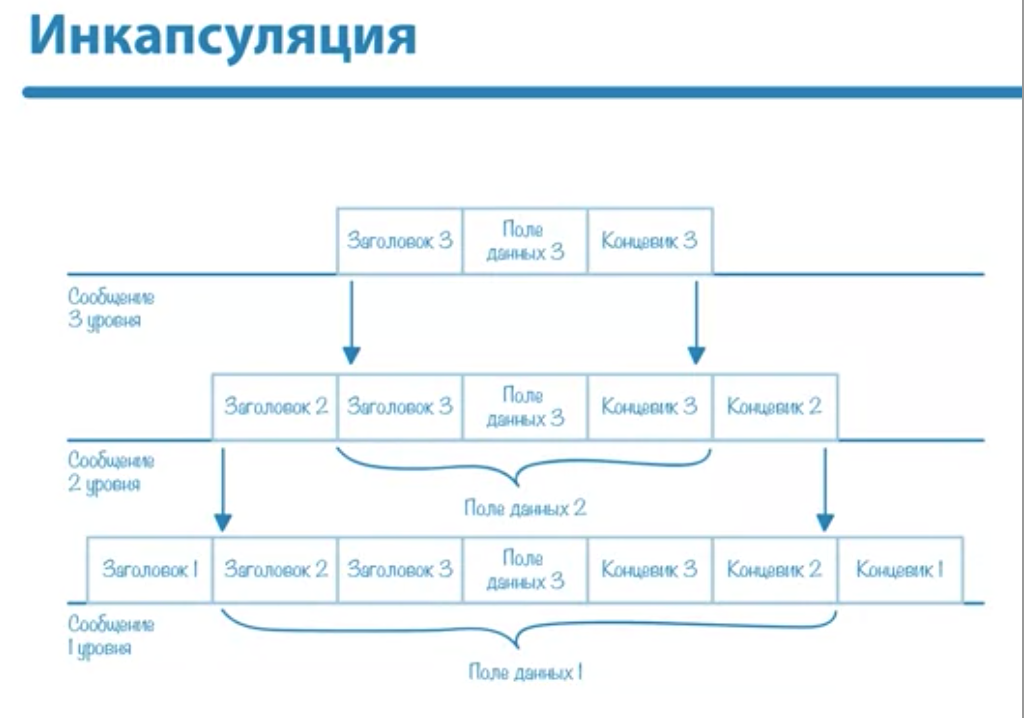
\includegraphics[scale = 0.4]{1.png}}
			\label{1}
		\end{center}
	\end{figure}

	После этого сообщение передается по каналам связи.
	
	Основные модели организации архитектуры сети:
	
	\begin{itemize}
		\item Модель взаимодействия открытых систем OSI;
		\item Модель TCP/IP.
	\end{itemize}

	\subsection{Урок 2:Модель TCP/IP и немного про модель OSI}
	
	\begin{figure}[h!]
		\begin{center}
			{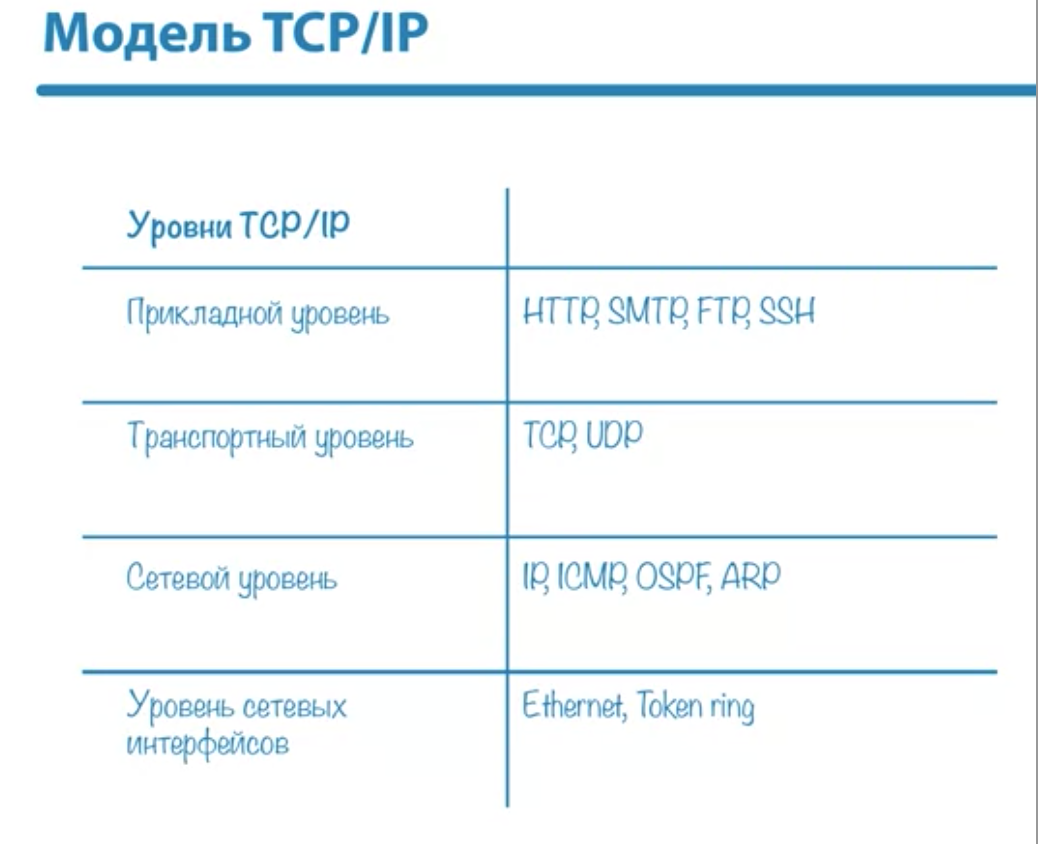
\includegraphics[scale = 0.4]{2.png}}
			\label{2}
		\end{center}
	\end{figure}


	\subsubsection{Уровень сетевых интерфейсов (Network access layer)}
	
	Задачи:
	
	\begin{itemize}
		\item упаковка IP-пакета в единицу передаваемых данных промежуточной сети;
		\item преобразование сетевых адресов в адреса технологии данной промежуточной сети.
	\end{itemize}

	\begin{figure}[h!]
		\begin{center}
			{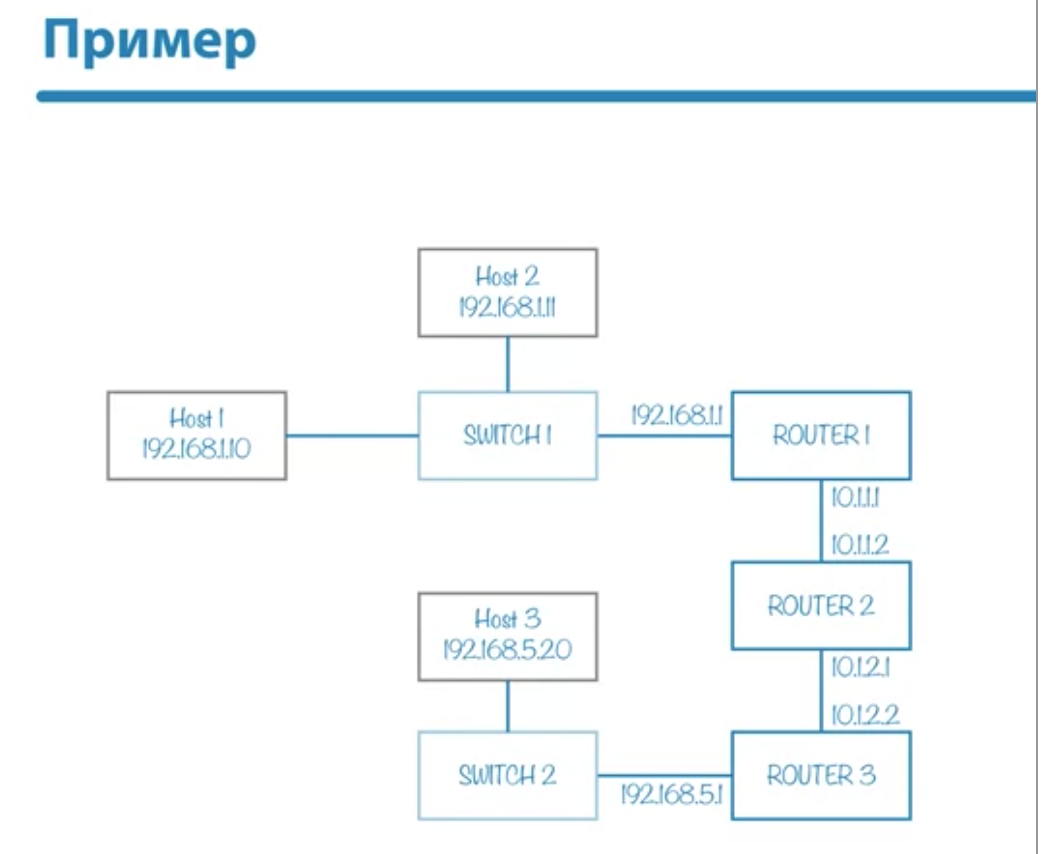
\includegraphics[scale = 0.4]{3.png}}
			\label{3}
		\end{center}
	\end{figure}

	Происходит преобразование IP-адреса в адрес локальной технологии (его mac-адрес). И с помощью этой локальной технологии пакет доставится адресату.
	
	\subsubsection{Сетевой уровень (Network layer)}
	
	\begin{itemize}
		\item Служит для образования единой транспортной системы, объединяющей несколько сетей, причем эти сети могут использовать совершенно разные технологии передачи данных;
		\item Пример протокола: IP.
	\end{itemize}

	Тот же пример, что и был. На этот раз необходимо доставить пакет от Host1 к Host3. Задача сетевого уровня - найти путь и доставить пакет от router 1 к router 3. Доставкой пакета от Host1 к Router1 и от Router3 к Host3 занимается локальная технология, например, <<изернет>>.
	
	Пример протокола сетевого уровня: IP.
	
	\subsubsection{Транспортный уровень (Transport layer).}
	
	Обеспечивает передачу данных между процессами (?).
	
	\begin{itemize}
		\item Особенностью транспортного уровня является управление надежностью. Уровенть предоставяет приложениям или верхним уровням стека передачу данных с той степенью надежности, которая им требуется.
		\item Примеры протоколов: TCP и UDP.
	\end{itemize}

	Пример: необходимо передать большой файл по сети. Он будет передаваться кусочками. Необходимо, чтобы каждый кусок дошел, да еще чтоб в правильном порядке.

	\subsubsection{Прикладной уровень (Application layer).}
	
	\begin{itemize}
		\item Набор разнообразных протоколов, с помощью которых пользователи сети получают доступ к разделяемым ресурсам.
		\item Пример протоколов: HTTP, FTP.
	\end{itemize}

	\subsubsection{Модель OSI (Open Systems Interconnection) (модель взаимодействия открытых систем).}
	
	\begin{figure}[h!]
		\begin{center}
			{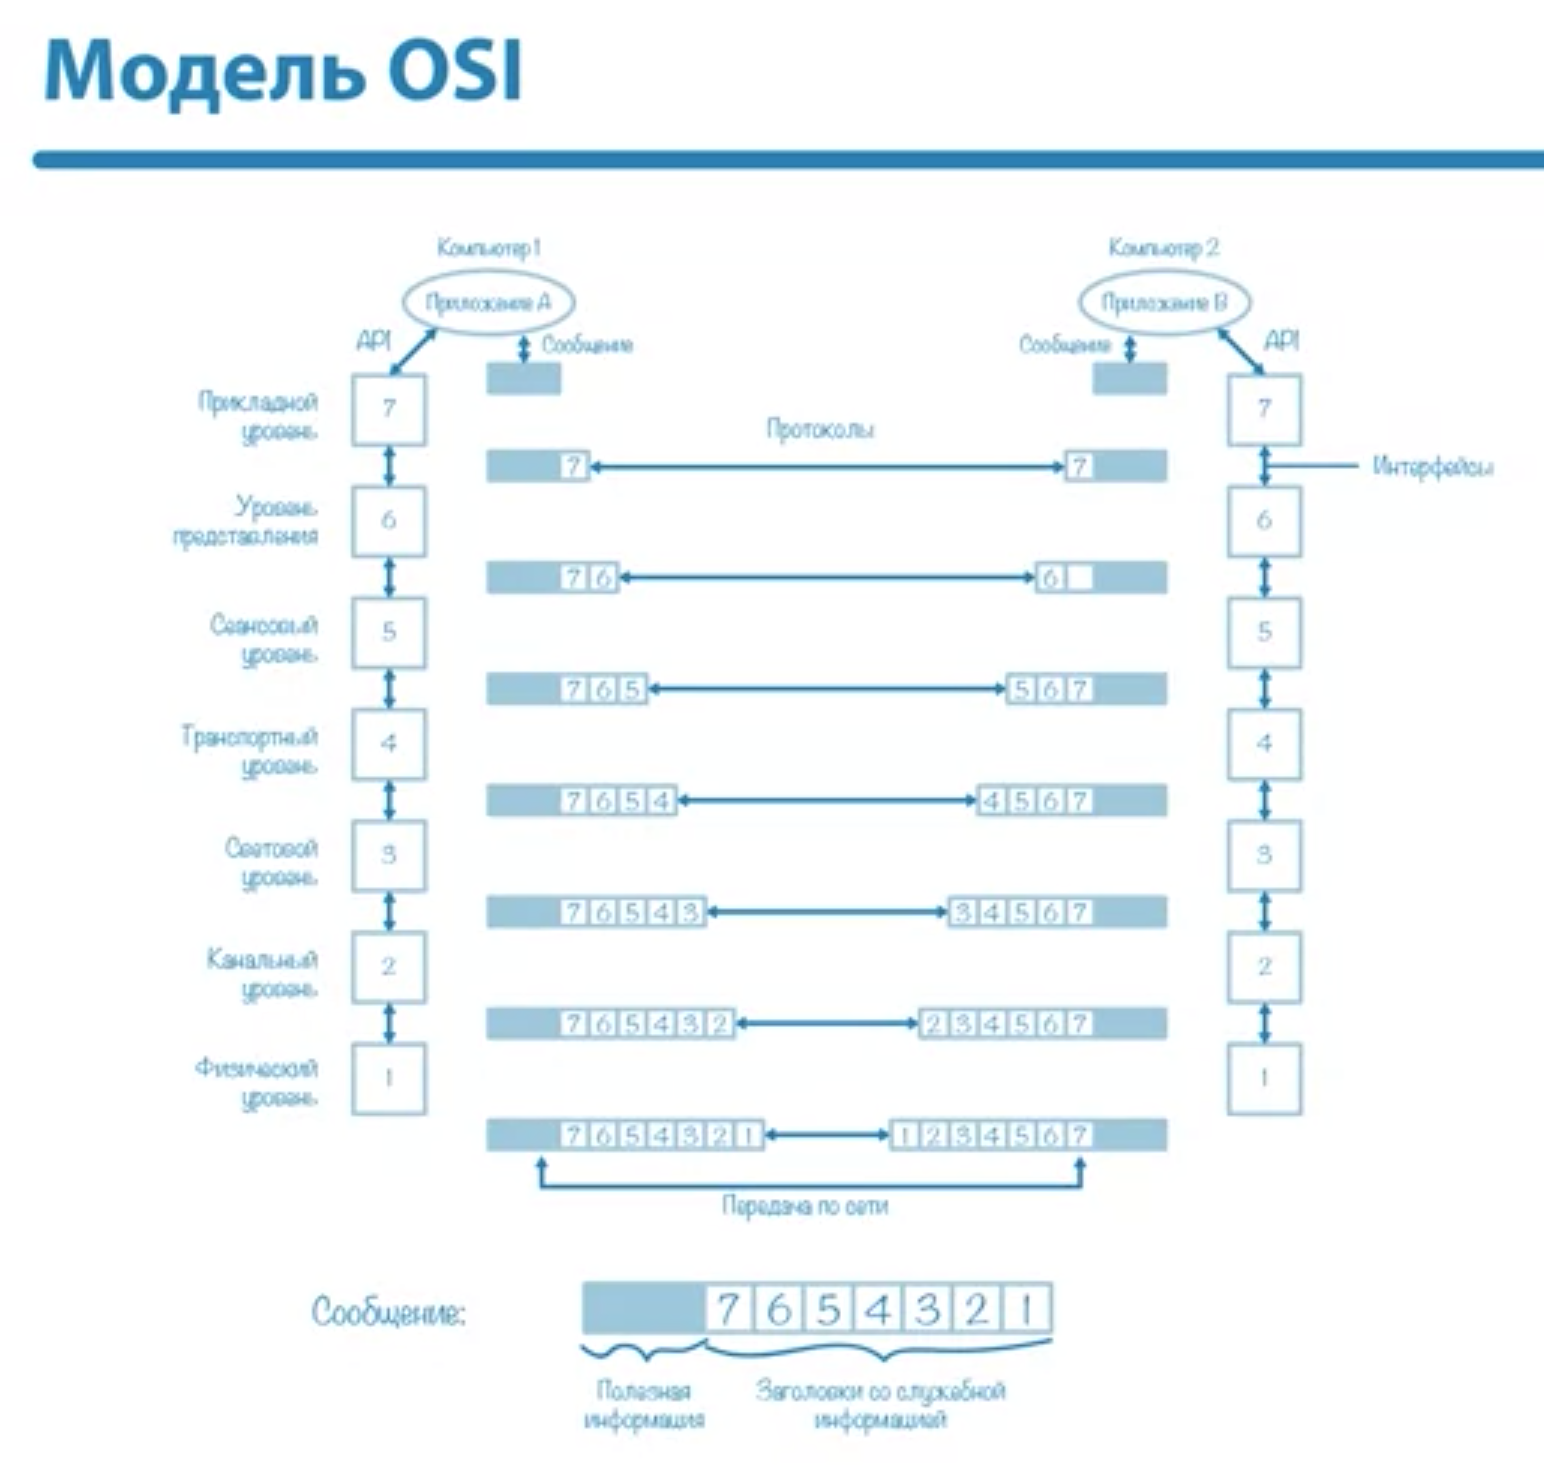
\includegraphics[scale = 0.4]{4.png}}
			\label{4}
		\end{center}
	\end{figure}
	
	Модель OSI и TCP/IP во многом схожи. Достоинство модели OSI - теоретически проработанна. Но на практике широко не применяется.
	Достоинство TCP/IP - стек протоколов. Тк он широко применяется на практике и лежит в основе интернета.
	
	\subsection{Урок 3: Детально транспортный уровень и его протоколы.}
	
	Задачи транспортного уровня
	
	\begin{itemize}
		\item передача данных между процессами в сети;
		\item предоставление различного уровня надежности передачи данных, независимо от надежности сети.
	\end{itemize}

	Для адресации на траспортном уровне используются порты.

	Каждое сетевое приложение на хосте имеет свой порт. Номера портов у приложений не должны повторяться.
	
	Формат записи вместе с IP-адресом:
	192.168.0.1:8080
	
	\subsubsection{Протокол UDP (User Datagram Protocol).}
	
	Особенности UDP:
	
	\begin{itemize}
		\item Работает без установления логического соединения;
		\item Нет гарантии доставки данных;
		\item Нет гарантии сохранения исходного порядка дейтаграмм;
		\item Гарантирует корректность данных внутри одной дейтаграммы.
	\end{itemize}

	\begin{figure}[h!]
		\begin{center}
			{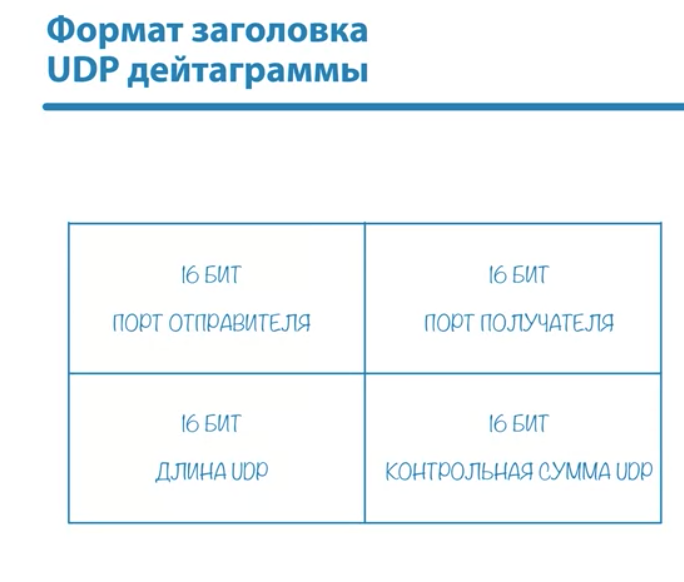
\includegraphics[scale = 1]{5.png}}
			\label{5}
		\end{center}
	\end{figure}

	
	\subsubsection{Протокол TCP (Transmission control protocol)}
		
	\begin{itemize}
		\item Является надежным протоколом передачи данных.
		\item Особенности TCP
		\begin{itemize}
			\item Работает с установления логического соединения
			\item Гарантирует доставку данных
			\item Гарантирует сохранение порядка следования пакетов
		\end{itemize}
	\end{itemize}
		
	\begin{figure}[h!]
		\begin{center}
			{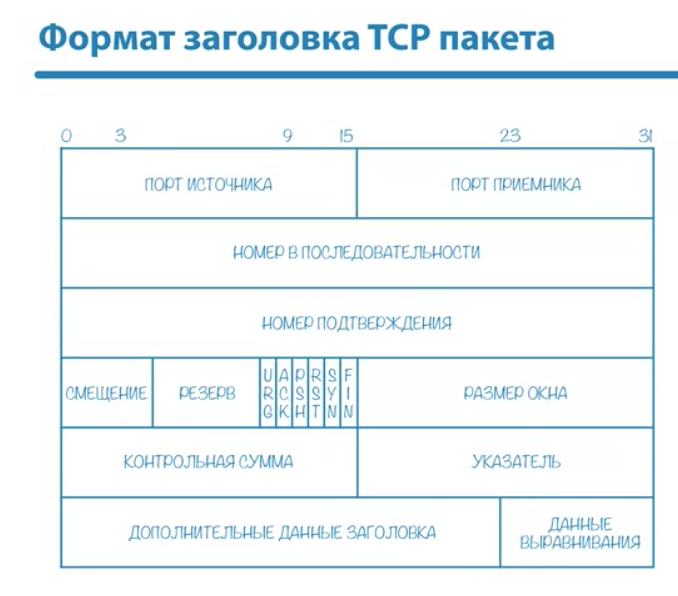
\includegraphics[scale = 1]{6.png}}
			\label{6}
		\end{center}
	\end{figure}

	\subsubsection{Логическое соединение}
	
	Для надежности передачи данных между двумя процессами необходимо установить логическое соединение. <<Соединение>> является договоренность о параметрах между двумя процессами.
	
	Взаимодействие партнеров с использованием протокола TCP строится в три этапа:
	
	\begin{itemize}
		\item установление логического соединения;
		\item обмен данными;
		\item закрытие соединения.
	\end{itemize}

	\begin{figure}[h!]
		\begin{center}
			{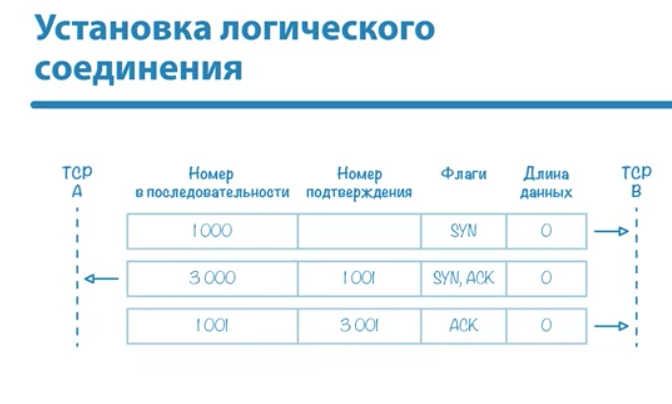
\includegraphics[scale = 0.8]{7.png}}
			\label{7}
		\end{center}
	\end{figure}

	Флаг SYN - пакет является запросом для установления логического соединения.
	
	TCP B отвечает в номере подтверждения на 1 больше чем в номере последовательности.
	
	Флаг ACK - означает, что TCP пакет содержит в своем поле номера подтверждения верные данные.
	
	На третьем шаге A подтверждает правильность приема пакета B.
	
	\subsubsection{Процесс обмена данными}
	
	\begin{figure}[h!]
		\begin{center}
			{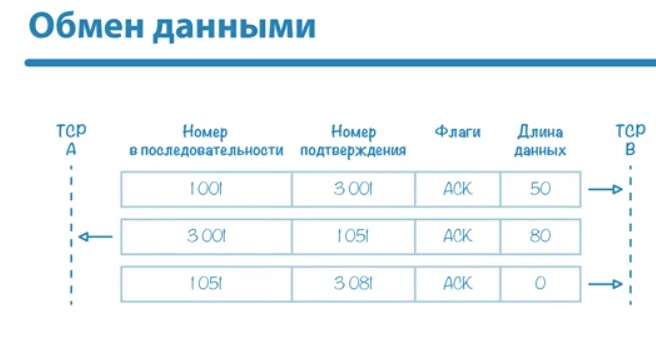
\includegraphics[scale = 1]{8.png}}
			\label{8}
		\end{center}
	\end{figure}

	Каждый раз когда TCP модуль принимает данные, он подтверждает их прием:
	
	вычисляет значение поля <<номер подтверждения>> = номер в последовательности + длина данных.
	
	
	\subsubsection{Закрытие соединения}
	
	По инициативе A:
	
	\begin{figure}[h!]
		\begin{center}
			{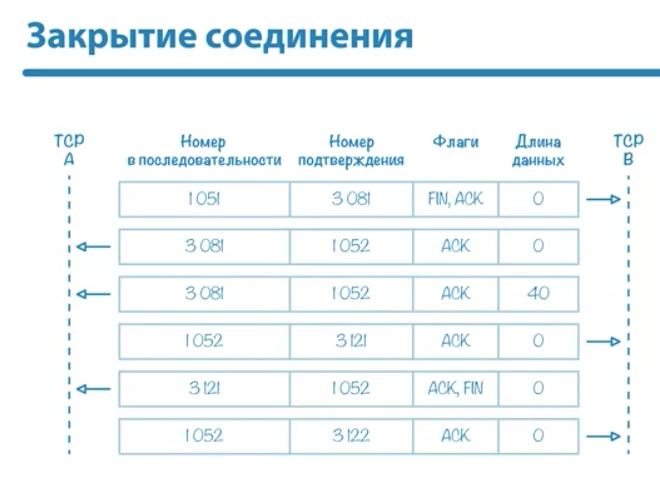
\includegraphics[scale = 1]{9.png}}
			\label{9}
		\end{center}
	\end{figure}

	Флаг FIN - Tcp пакет представляет из себя запрос на закрытие логического соединения и вляется признаком конца потока данных.
	
	B отправляет пакет, у которого в номере подтверждения на 1 больше значение чем в номере последовательности полученного от A.
	
	После этого посылка данных от A невозможна, но B имеет возможность отправлять данные A и получать подтверждение об этом.
	
	После того как пакет B формирует флаг FIN и получает подтверждение о его принятии, соединение считается закрытым.
	
	\subsection{Протоколы UDP и TCP на практике}
	
	seq - номер в последовательности
	
	win - размер окна (?)
	
	флаг S - SYN
	
	флаг . - ACK
	
	Флаги E, W - служебные флаги.
	
	ack - номер подтверждения.
	
	дальше идут номера последовательности в относительном режиме (от единицы) пример: 1:15.
	
	Флаг F - FIN.
	
	\subsection{DNS-протокол}
	
	DNS (Domain Name System - система доменных имен) - распределенная система для получения информации о доменах. Чаще всего используется для получения IP-адреса по имени хоста (компьютера или устройства).
	
	Раньше было так:
	
	\begin{figure}[h!]
		\begin{center}
			{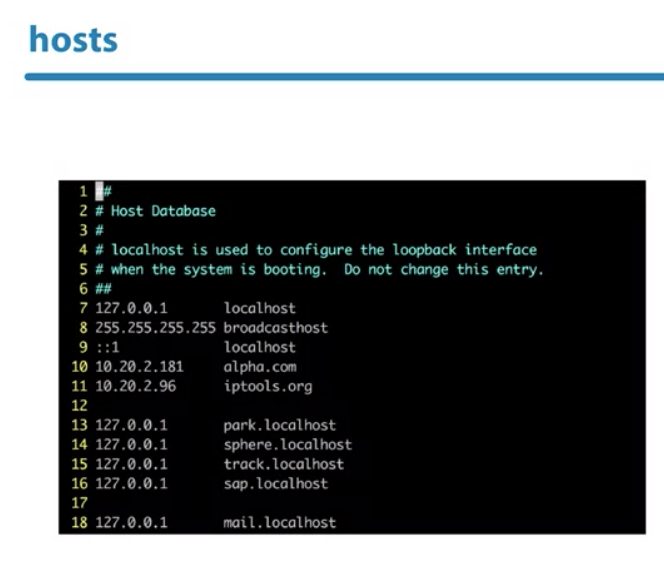
\includegraphics[scale = 1]{10.png}}
			\label{10}
		\end{center}
	\end{figure}

	Потом он стал слишком большим и придумали DNS.
	
	\subsubsection{Назначение DNS}
	
	Распределенность. Ответственность за разные части иерархической структуры несут разные люди или организации; каждый узел сетив обязательном порядке должен хранить только те данные, которые входят в его зону ответственности.
	
	Кэширование. Узел может хранить некоторое количество данных не из своей зоны ответственности для уменьшения нагрузки на сеть.
	
	Резервирование. За хранение и обслуживание своих узлов (зон) отвечают (обычно) несколько серверов.
	
	\subsubsection{Структура DNS}
	
	\begin{figure}[h!]
		\begin{center}
			{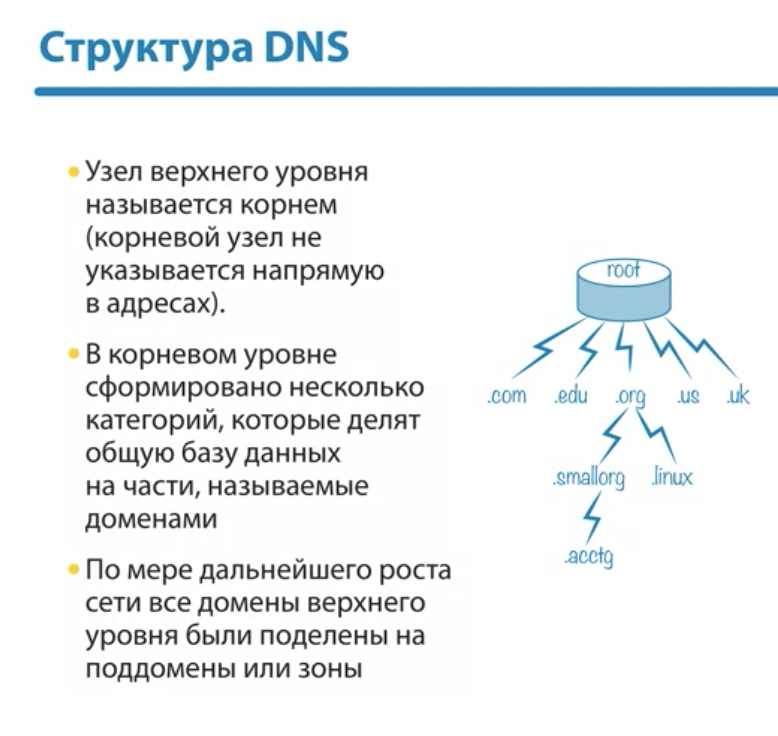
\includegraphics[scale = 1]{11.png}}
			\label{11}
		\end{center}
	\end{figure}
	
	\subsubsection{Схемы разрешения DNS-имен}
	
	{\bf Нерекурсивная.}
	
	Клиент обращается к корневому DNS-серверу с указанием полного доменного имени, он отвечает клиенту, указывая адрес следующего DNS-сервера. Клиент делает запрос следующего DNS-сервера, который отсылает к DNS-серверу нужного поддомента и т.д., пока не будет найден DNS-сервер, в котором хранится соответствие запрошенного имени IP-адресу. Этот сервер дает окончательный ответ клиенту.
	
	{\bf Рекурсивная.}
	
	Клиент запрашивает локальный DNS-сервер. Далее возможны два варианта действий: если локальный DNS-сервер знает ответ, то он сразу же возвращает его клиенту; если локальный сервер не знает ответ, то он выполняет итеративные запросы к корневому серверу и т.д. точно так же, как это делал клиент в предыдущем варианте, а подучив ответ, передает его клиенту, который все это время просто эжет его от своего DNS-сервера.
	
	\subsubsection{Типы записей в DNS}
	
	DNS-сервер, отвечающий за имена хостов в своей зоне, должен хранить информацию о хостах в базе данных и выдавать е по запросу с удаленных компьютеров. Обычно, база данных DNS представляет собой текстовый файл, состоящий из исходных записей RR (resource records).
	
	Записи:
	
	\begin{itemize}
		\item A-запись.
		
		Указывает адрес хоста. Она отображает хост-имя на адрес и может выглядеть следующим образом: myhost.mycompany.com IN A 192.168.0.1
		\item AAAA-запись.
		
		Указывает адрес хоста. Она отображает хост-имя на адрес IPv6 и может выглядеть следующим образом:
		
		myhost.mycompany.com IN AAAA 1234:1:2:3:4:567:89cd
		\item CNAME-запись
		
		Это каноническая запись, обычно используемая для алиасов (псевдонимов). Она позволяет отображать несколько хост-имен на заданный IP-адрес.
		\item NS-запись.
		
		В каждой зоне должно быть по крайней мере два сервера DNS. Записи NS служат для их идентификации другими DNS-серверами, которые пытаются преобразовать имена хостов, относящихся к данной зоне.
		\item SOA-запись.
		
		Запись, которая определяет авторитетную информацию о DNS-зоне.
		
		Например, указываются параметры:
		\begin{itemize}
			\item Primary Name Server - имя первичного DNS-сервера зоны
			\item Hostmaster - контактный адрес лица, ответственного за администрирование файла зоны
			\item Serial number - серийный номер файла зоны. 32-разрядное целое число, меняющееся при каждом обновлении зоны.
		\end{itemize}
		\item PTR-запись
		
		Запись позволяет быстро выполнять обратный поиск с помощью зоны обратного поиска (inaddr.arpa). Она считается обратной A-записью, но не похожа на нее ввиду использования inaddr.arpa в реальной записи.
		
		Такая запись для хоста syscrusher.skillet.com с IP-адресом 100.200.252.1 имеет следующий вид: 1.252.200.100.in-addr.arpa IN PTR syscrusher.skillet.com.
		\item MX-запись
		
		С их помощью удаленные серверы электронной почты узнают, куда отправлять почту для вашей зоны.
		\item TXT-запись
		
		Запись TXT содержит текстовые данные любого вида.
	\end{itemize}
	
	\subsubsection{Утилита dig}
	
	-x - ищет PTR записи по IP-адресу.
	
	mx - mx записи дополнительно
	
	+trace - то, как происходит поиск нужного IP-адреса (его путь).
	
	\subsection{HTTP-протокол}
	
	\subsubsection{HTTP-протокол}
	
	HTTP (HyperText Transfer Protocol - RFC 1945, RFC 2616) - протокол прикладного уровня для передачи гипертекста.
	
	Все ПО для работы с протоколом HTTP разделяется на:
	
	\begin{itemize}
		\item Сервер - поставщики услуг хранения и обработки информации (обработка запросов).
		\item Клиент - конечные потребители услуг сервера (отправка запросов).
	\end{itemize}
	
	\subsubsection{Схема HTTP-сеанса}
	
	\begin{itemize}
		\item Установление TCP-соединения.
		\item Запрос клиента.
		\item Ответ сервера.
		\item Разрыв TCP-соединения.
	\end{itemize}
	
	Таким образом, клиент посылает серверу запрос, получает от него ответ, после чего взаимодействие прекращается. Из этого следует, что протокол не хранит информацию о предыдущих запросах клиентов и ответах сервера.
	
	\subsubsection{URI/URL}
	
	\textit{Для того, чтобы получить какие-то данные, необходимо КУДА-ТО за ними сходить}
	
	Единообразный идентификатор ресурса URI (Uniform Resource Identifier) представляет собой короткую последовательность символов, идентифицирующую абстрактный или физический ресурс. URI не указывает на то, как получить ресурс, а только идентифицирует его. Один из самых известных примеров URI - URL.
	
	Для однозначной идентификации ресурсов в сети Веб используются уникальные идентификаторы URL (Uniform Resource Locator). \textit{Указывает однозначно - где находится ресурс и как его получить.}
	
	Имеет следующую структуру:
	
	<схема>://<логин>:<пароль>@<хост>:<порт>/<URL-путь>.
	
	схема это - http, ftp, https и тд.
	
	логин и пароль - необязательные поля, которые в каких-то протоколах требуются, а в каких-то нет (в http они опускаются).
	
	хост и порт к которым нужно обратиться
	
	
	
	\subsubsection{Структура запроса}
	
	\begin{figure}[h!]
		\begin{center}
			{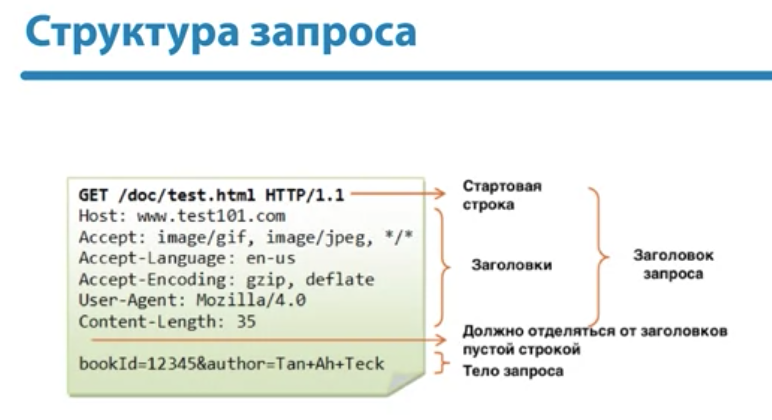
\includegraphics[scale = 1]{12.png}}
			\label{12}
		\end{center}
	\end{figure}

	{\bf Стартовая строка HTTP}
	
	Стартовая строка является обязательным элементом, так как указывает на тип запроса/ответа, заголовки и тело сообщения могут отсутствовать. Стартовые строки различаются для запроса и ответа.
	
	Строка запроса выглядит так:
	Метод URL-Путь HTTP/Версия протокола
	
	\subsubsection{Виды запросов}
	
	{\bf Методы протокола:}
	\begin{itemize}
		\item GET
		
		Используется для получения какой-то информации (пример: мы делаем запрос в браузере).
		\item HEAD
		
		Аналогично GET, но он как бы говорит:\textit{выполни запрос, но не присылай тело этого запроса (?)}
		\item POST
		
		Служит, чтобы отсылать от клиента данные на сервер.
		\item PATCH.
		
		Служит для того, чтобы изменять отправленные данные.
		Пример: С помощью POST мы отправили какую-то информацию на сервер, она сохранилась и теперь, чтоб изменить ее мы используем PATCH.
		\item DELETE
		
		Обращаемся к серверу с необходимостью удалить какие-то данные.
		
		\item PUT
		
		\item ...
	\end{itemize}

	PATCH используется для частичного изменения ресурса. PUT создает новый ресурс или заменяет представление целевого ресурса, данными представленными в теле запроса.

	{\bf Поля заголовка}
	
	Поля заголовка, следующие за строкой состояния, позволяют уточнять запрос т.е. передавать серверу дополнительную информацию. Поле заголовка имеет следующий формат:
	
	Имя\_поля:Значение.
	
	\textit{Различные поля заголовка:}
	\begin{itemize}
		\item Host - доменное имя или IP-адрес узла, к которому обращается клиент
		\item Referer - URL, откуда перешел клиент (например, если мы с google.com перешли на docs.google.com, то в Reger будет передаваться google.com)
		\item Accept - MIME-типы данных, обрабатываемых клиентом.
		\item Accept-Charset - перечень поддерживаемых кодировок
		\item Content-Type - MIME-тип данных, содержащихся в теле запроса
		\item Content-Length - число символов, содержащихся в теле запроса
		\item Connection - дирректива для управления TCP-соединением (например, если в Connection указать тип Live, то соединение не будет закрыто и будет использовано для дальнейших запросов)
		\item User-Agent - информация о клиенте (например, если мы делаем запрос с мозилы, то в User-agent отобразится это, если с сафари, то с сафари и тд)
	\end{itemize}

	{\bf MIME}
	
	\textit{Данный спефицикатор позволяет передавать от клиента к серверу различные типы данных}
	
	Спецификация MIME (Multipurpose Internet Mail Extension - многоцелевое почтовое расширение Internet) первоначально была разработана для того, чтобы обеспечить передачу различных форматов данных в составе электронных писем.
	
	До появления MIME-устройства, взаимодействующие по протоколу HTTP, обменивались исключительно текстовой информацией.
	
	Для описания формата данных используются тип и подтип. Тип определяет. к какому классу относится формат содержимого HTTP-запроса или HTTP-ответа. Подтип уточняет формат (text/html, image/png)
	
	\subsubsection{Структура ответа}
	
	\begin{figure}[h!]
		\begin{center}
			{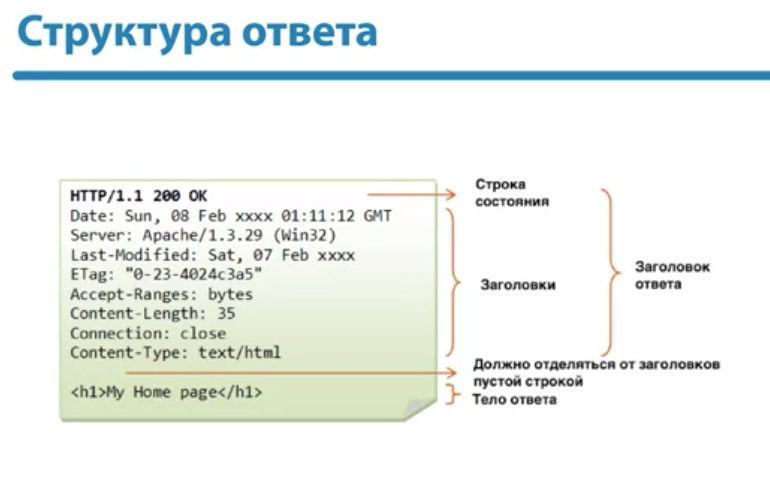
\includegraphics[scale = 1]{13.png}}
			\label{13}
		\end{center}
	\end{figure}
	
	Строка состояния состоит из версии протокола и статуса HTTP-ответа и расшифровки этого ответа.
	
	\subsubsection{Виды кодов (статусов) ответа}
	
	Существует 5 классов ответов:
	\begin{itemize}
		\item 1xx - специальный класс сообщений, называемых информационными.
		
		Означает, что сервер продолжает обработку запроса. (101 Switching Protocols) (например, мы работали по протоколу HTTP, а сервер нас переключил на работу по протоколу WEB-socket и для этого он отправляет статус 101)
		\item 2xx - успешная обработка запроса клиента. (пример 200 Ok - получаем этот статус. когда обращаемся к google.com и нам выдается страница; пример 201 Created - мы отправили на сервер какие-то данные, он их принял, сохранил и написал Created).
		\item 3xx - перенаправление запроса (301 Moved Permanently - в случае когда мы обращаемся к какому-то ресурсу, но этот ресурс переехал на другой адрес и нам сервер ответит 301; 302 Found - в случае если он также переехал но на какое-то время или же мы находились на /login, ввели правильно логин и пароль, он нас зарегестрировал и отправил на главную).
		\item 4xx - ошибка клиента. (400 Bad Request - некорректный HTTP-запрос; 403 Forbidden - недостаточно прав для доступа к ресурсу; 404 Not Found - обращение к ресурсу, которого не существует)
		\item 5xx - ошибка сервера. (500 Inernal Server Error - в том случае, когда логика сервера как-то некорректно отработала; 502 Bad Gateway - в случае, если вы, например, создали такую систему, в которой вначале клиент обращается к промежуточному серверу, а потом к вашему сервер-приложению и ващ сервер-приложение по какой-то причине не отвечает, то промежуточный сервер вернет 502)
	\end{itemize}

	\subsubsection{Основные заголовки}

	{\bf Поля заголовка ответа}
	\begin{itemize}
		\item Server - имя и номер версии сервера (пример: NGINX, Apache)
		\item Allow -  список методов, допустимых для данного ресурса
		\item Content-Type - MIME-тип данных, содержащихся в теле ответа сервера
		\item Content-Length - число символов, содержащихся в теле ответа сервера
		\item Last-Modified - дата и время последнего изменения ресурса
		\item Expires - дата и время, когда информация станет устаревшей
		\item Location - расположение ресурса (данный заголовок используется, например тогда, когда сервер нам прислал статус 302 и говорит нам переместиться на другой ресурс, соответственно, оттуда бразуер возьмет информацию и перейдет на другой ресурс)
		\item Cache-Control - директива управления кэшированием. (например, если указать в Cache-Control - NoCache, то данные которые приходят с сервера, никогда не будут сохранены или закэшированы).
	\end{itemize}
	
	
	
	\subsection{Регулярные выражения}
	
	\begin{figure}[h!]
		\begin{center}
			{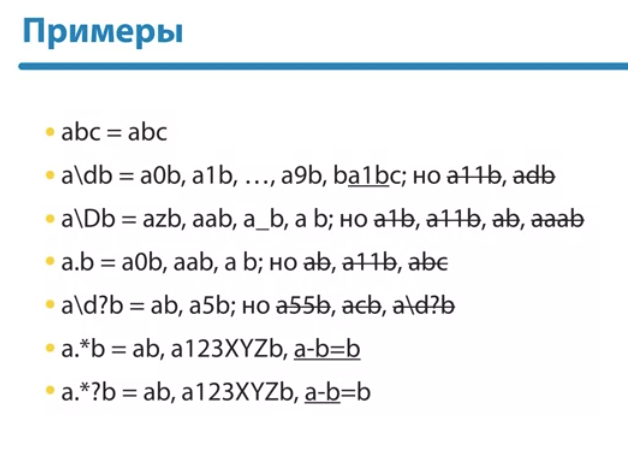
\includegraphics[scale = 1]{14.png}}
			\label{14}
		\end{center}
	\end{figure}
	
	\begin{figure}[h!]
		\begin{center}
			{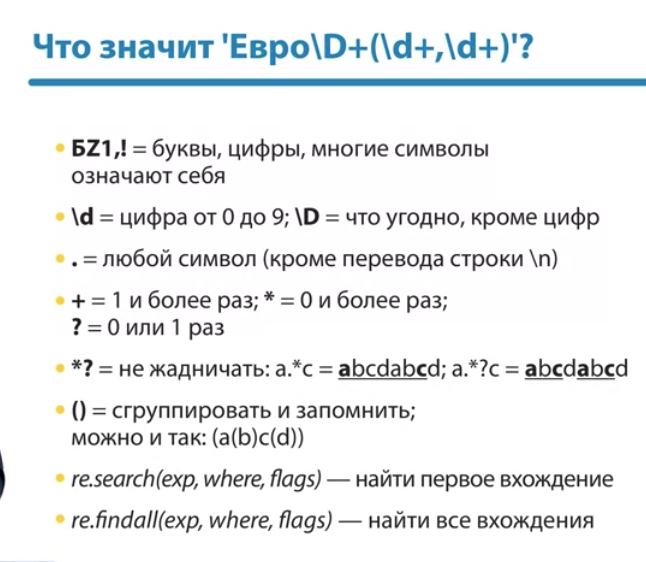
\includegraphics[scale = 1]{15.png}}
			\label{15}
		\end{center}
	\end{figure}
	
	\subsubsection{Символьные классы и квантификаторы}
	
	\begin{figure}[h!]
		\begin{center}
			{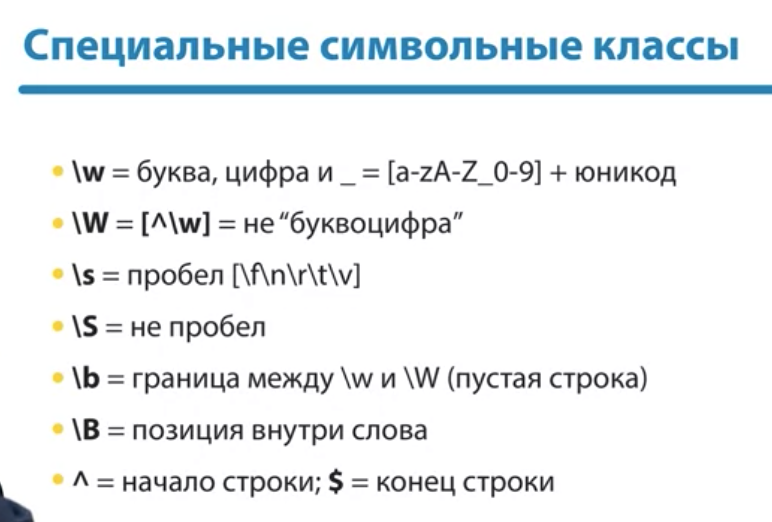
\includegraphics[scale = 1]{16.png}}
			\label{16}
		\end{center}
	\end{figure}

	\begin{figure}[h!]
		\begin{center}
			{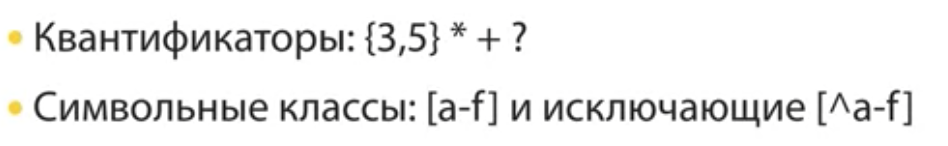
\includegraphics[scale = 1]{17.png}}
			\label{17}
		\end{center}
	\end{figure}

	\subsubsection{Сложный поиск и замена}
	
	{\bf Специальные символьные классы} - наиболее часто используемые символьные классы.
	
	\begin{figure}[h!]
		\begin{center}
			{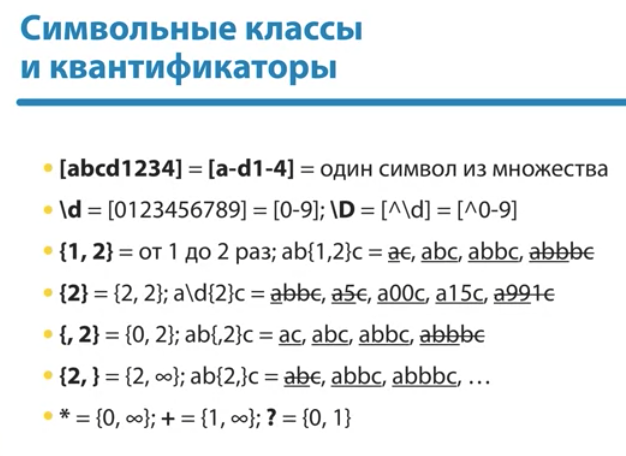
\includegraphics[scale = 1]{18.png}}
			\label{18}
		\end{center}
	\end{figure}
	
	Чтобы были только буквы латинского алфавита, необходимо установить флаг re.ASCII.
	
	Если указан флаг re.MULTILINE - то <<крышка>> и \$ означают начало и конец КАЖДОЙ строки.
	
	
		
	
\end{document}